\section{Problem Setup}

We base our environment setting on Breyer et al.'s table cleaning grasping environment. In the simulation environment, a gripper is spawned until the wrist and attempts to grasp randomly drawn objects from the table or the floor. The gripper is deprived of an arm and a base. Accordingly, the computation of inverse kinematics is ignored.

The observed state originates from the RGBD camera mounted on the gripper. The gripper is position controlled with continuous input between -1 to 1. Based on the task description, an action is represented either by [dx, dy, dz, \(\phi\), gripper open/close] or [dx, dy, \(\phi\)]. 

Episode either terminates by the timeout signal after 150 timesteps or the success signal. Success signal is triggered when the gripper carries an object to a predefined height defined by the curriculum strategy.

We conduct our experiments on two different simulation scenes: Floor (\ref{fig:table}) and table with a tray (\ref{fig:floor}). Floor scene represents the Breyer et al.'s setup, and the table with a tray scene is same as the Quillen et al.'s configuration. We investigated the transfer performance of the model trained in the floor scene in the table setup.

Different task descriptions will be explained in the next section. Our assumptions regarding the environment are:

\begin{enumerate}
    \item Gravity is compensated on the gripper, but not the objects.
    \item The gripper can only take relative action to its position. In every timestep, relative translation and rotation are limited to maximum of 3cm and 15cm, respectively.
    \item Other than applied actions, no other external force acts on the gripper. 
\end{enumerate}

\begin{figure}

    \begin{subfigure}{0.49\textwidth}
      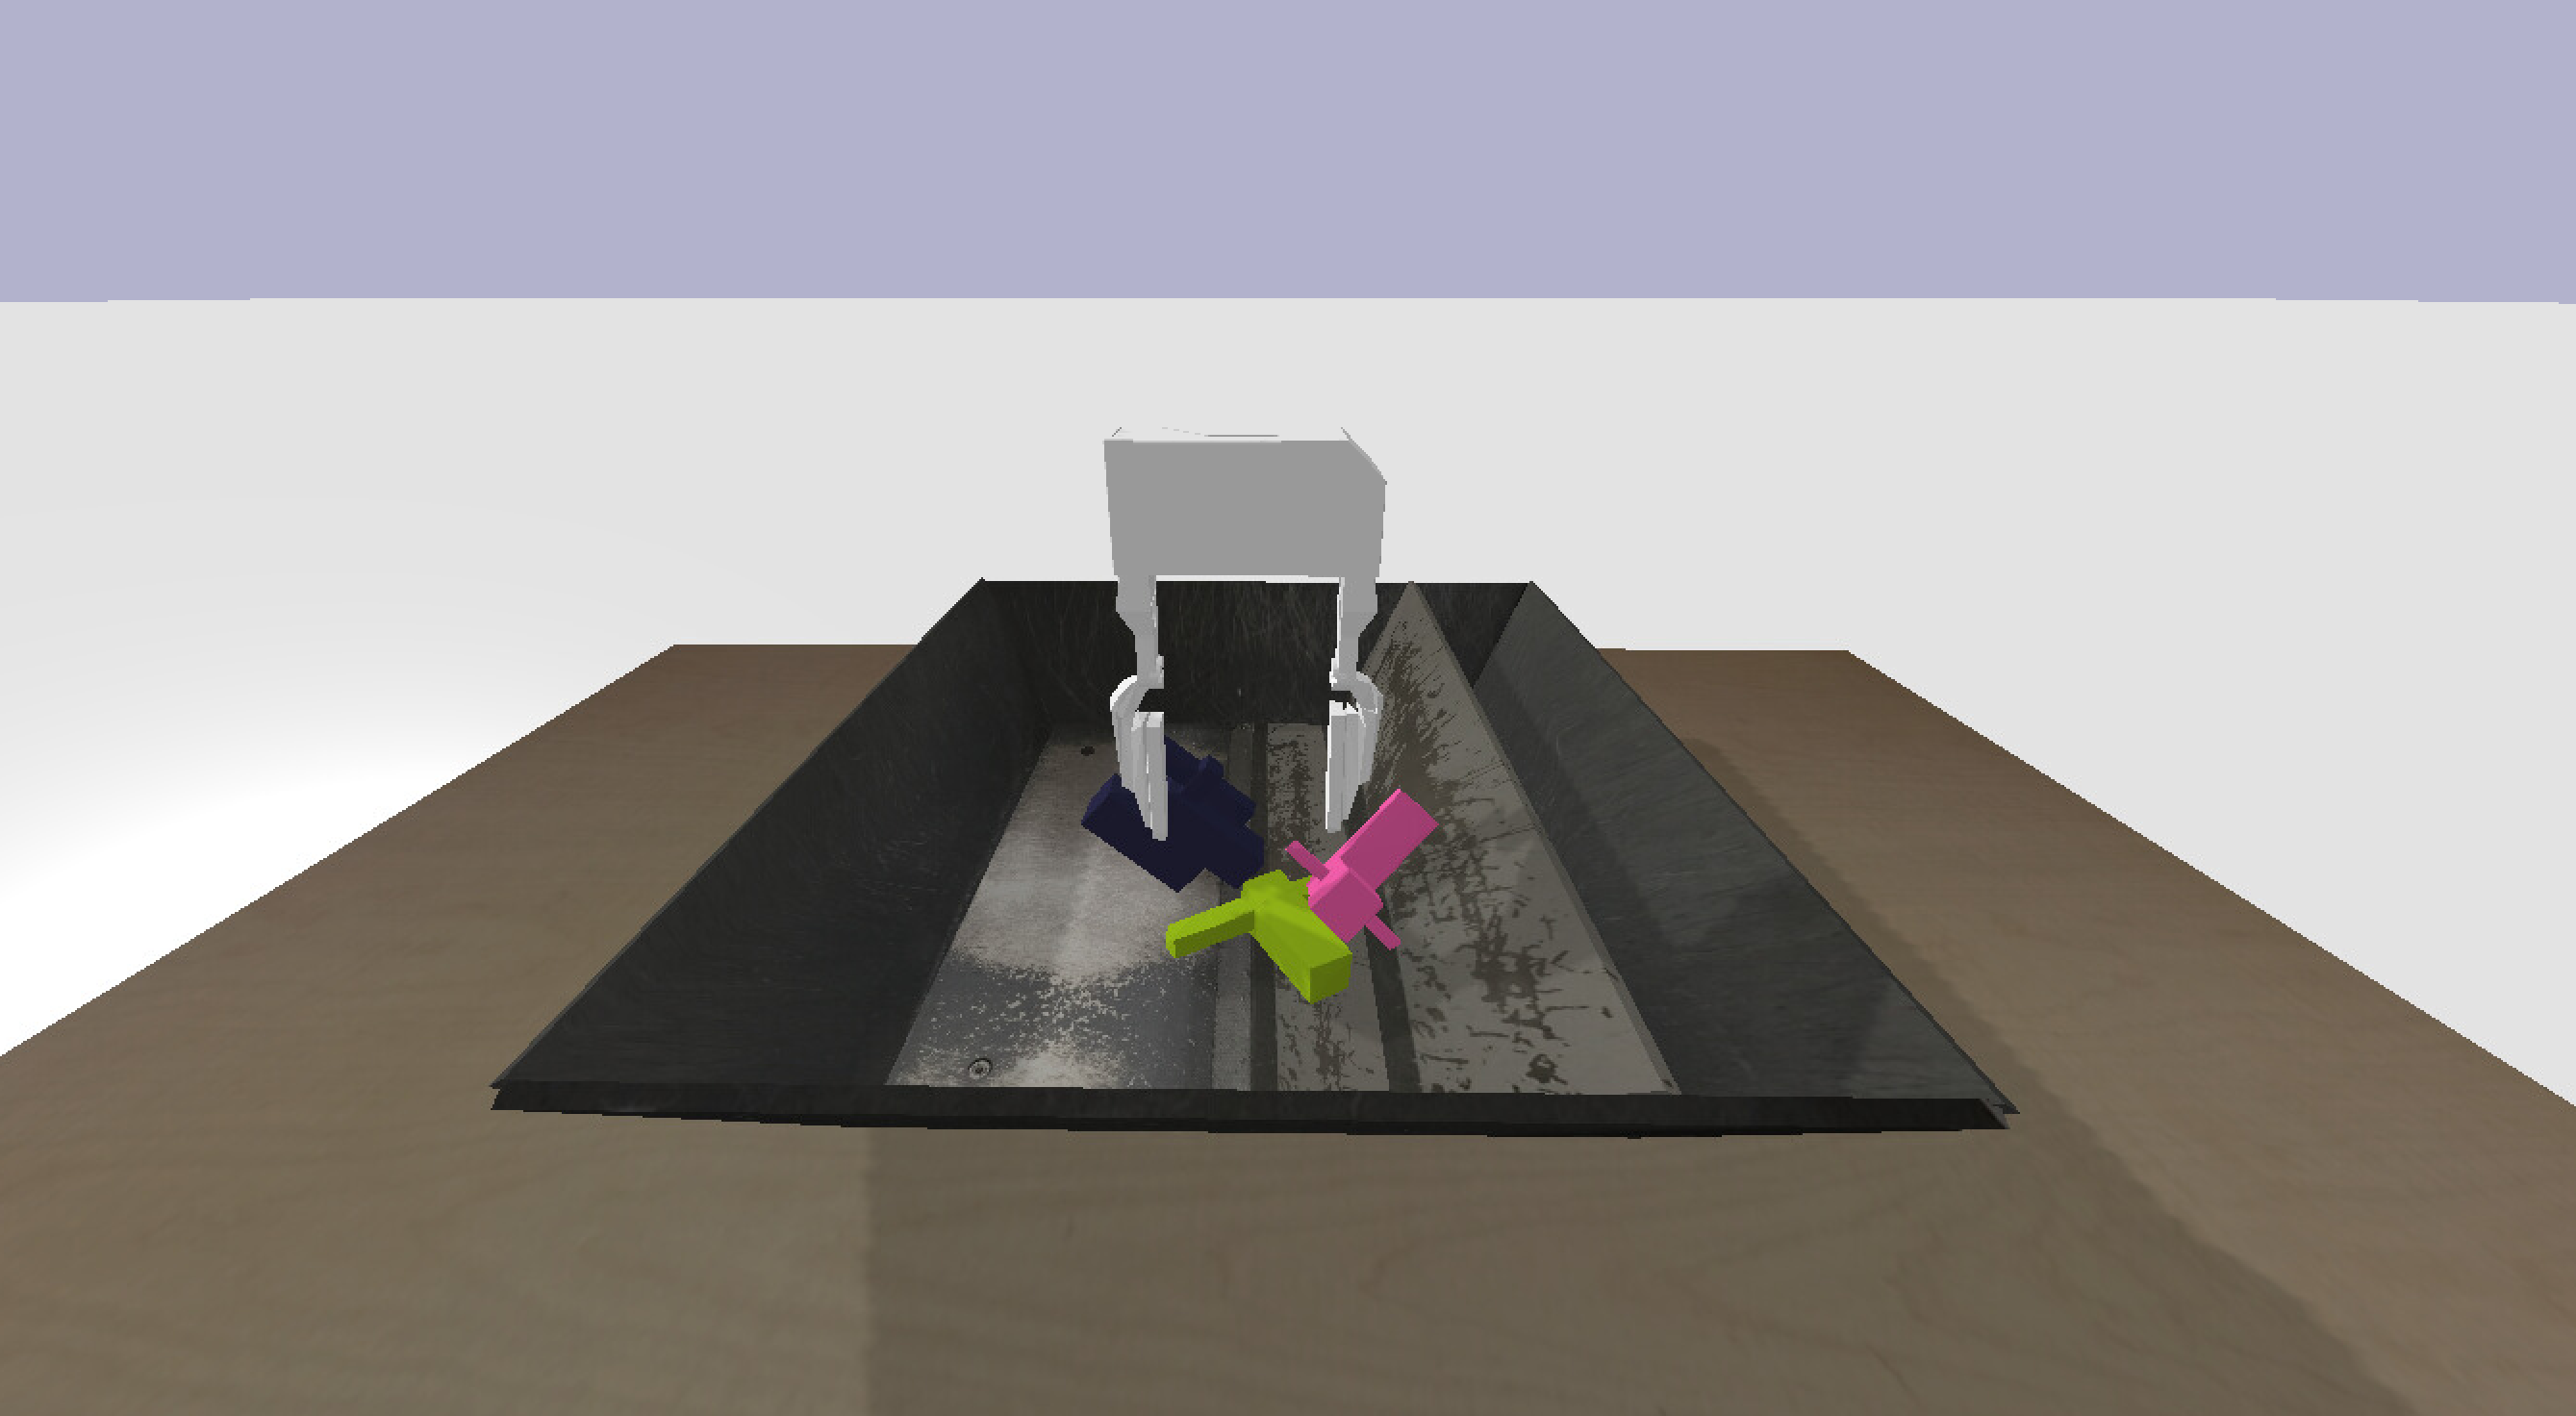
\includegraphics[width=\linewidth]{figures/tray.png}
      \caption{Table Scene} \label{fig:table}
    \end{subfigure}%
    \hspace*{\fill}   % maximize separation between the subfigures
    \begin{subfigure}{0.49\textwidth}
      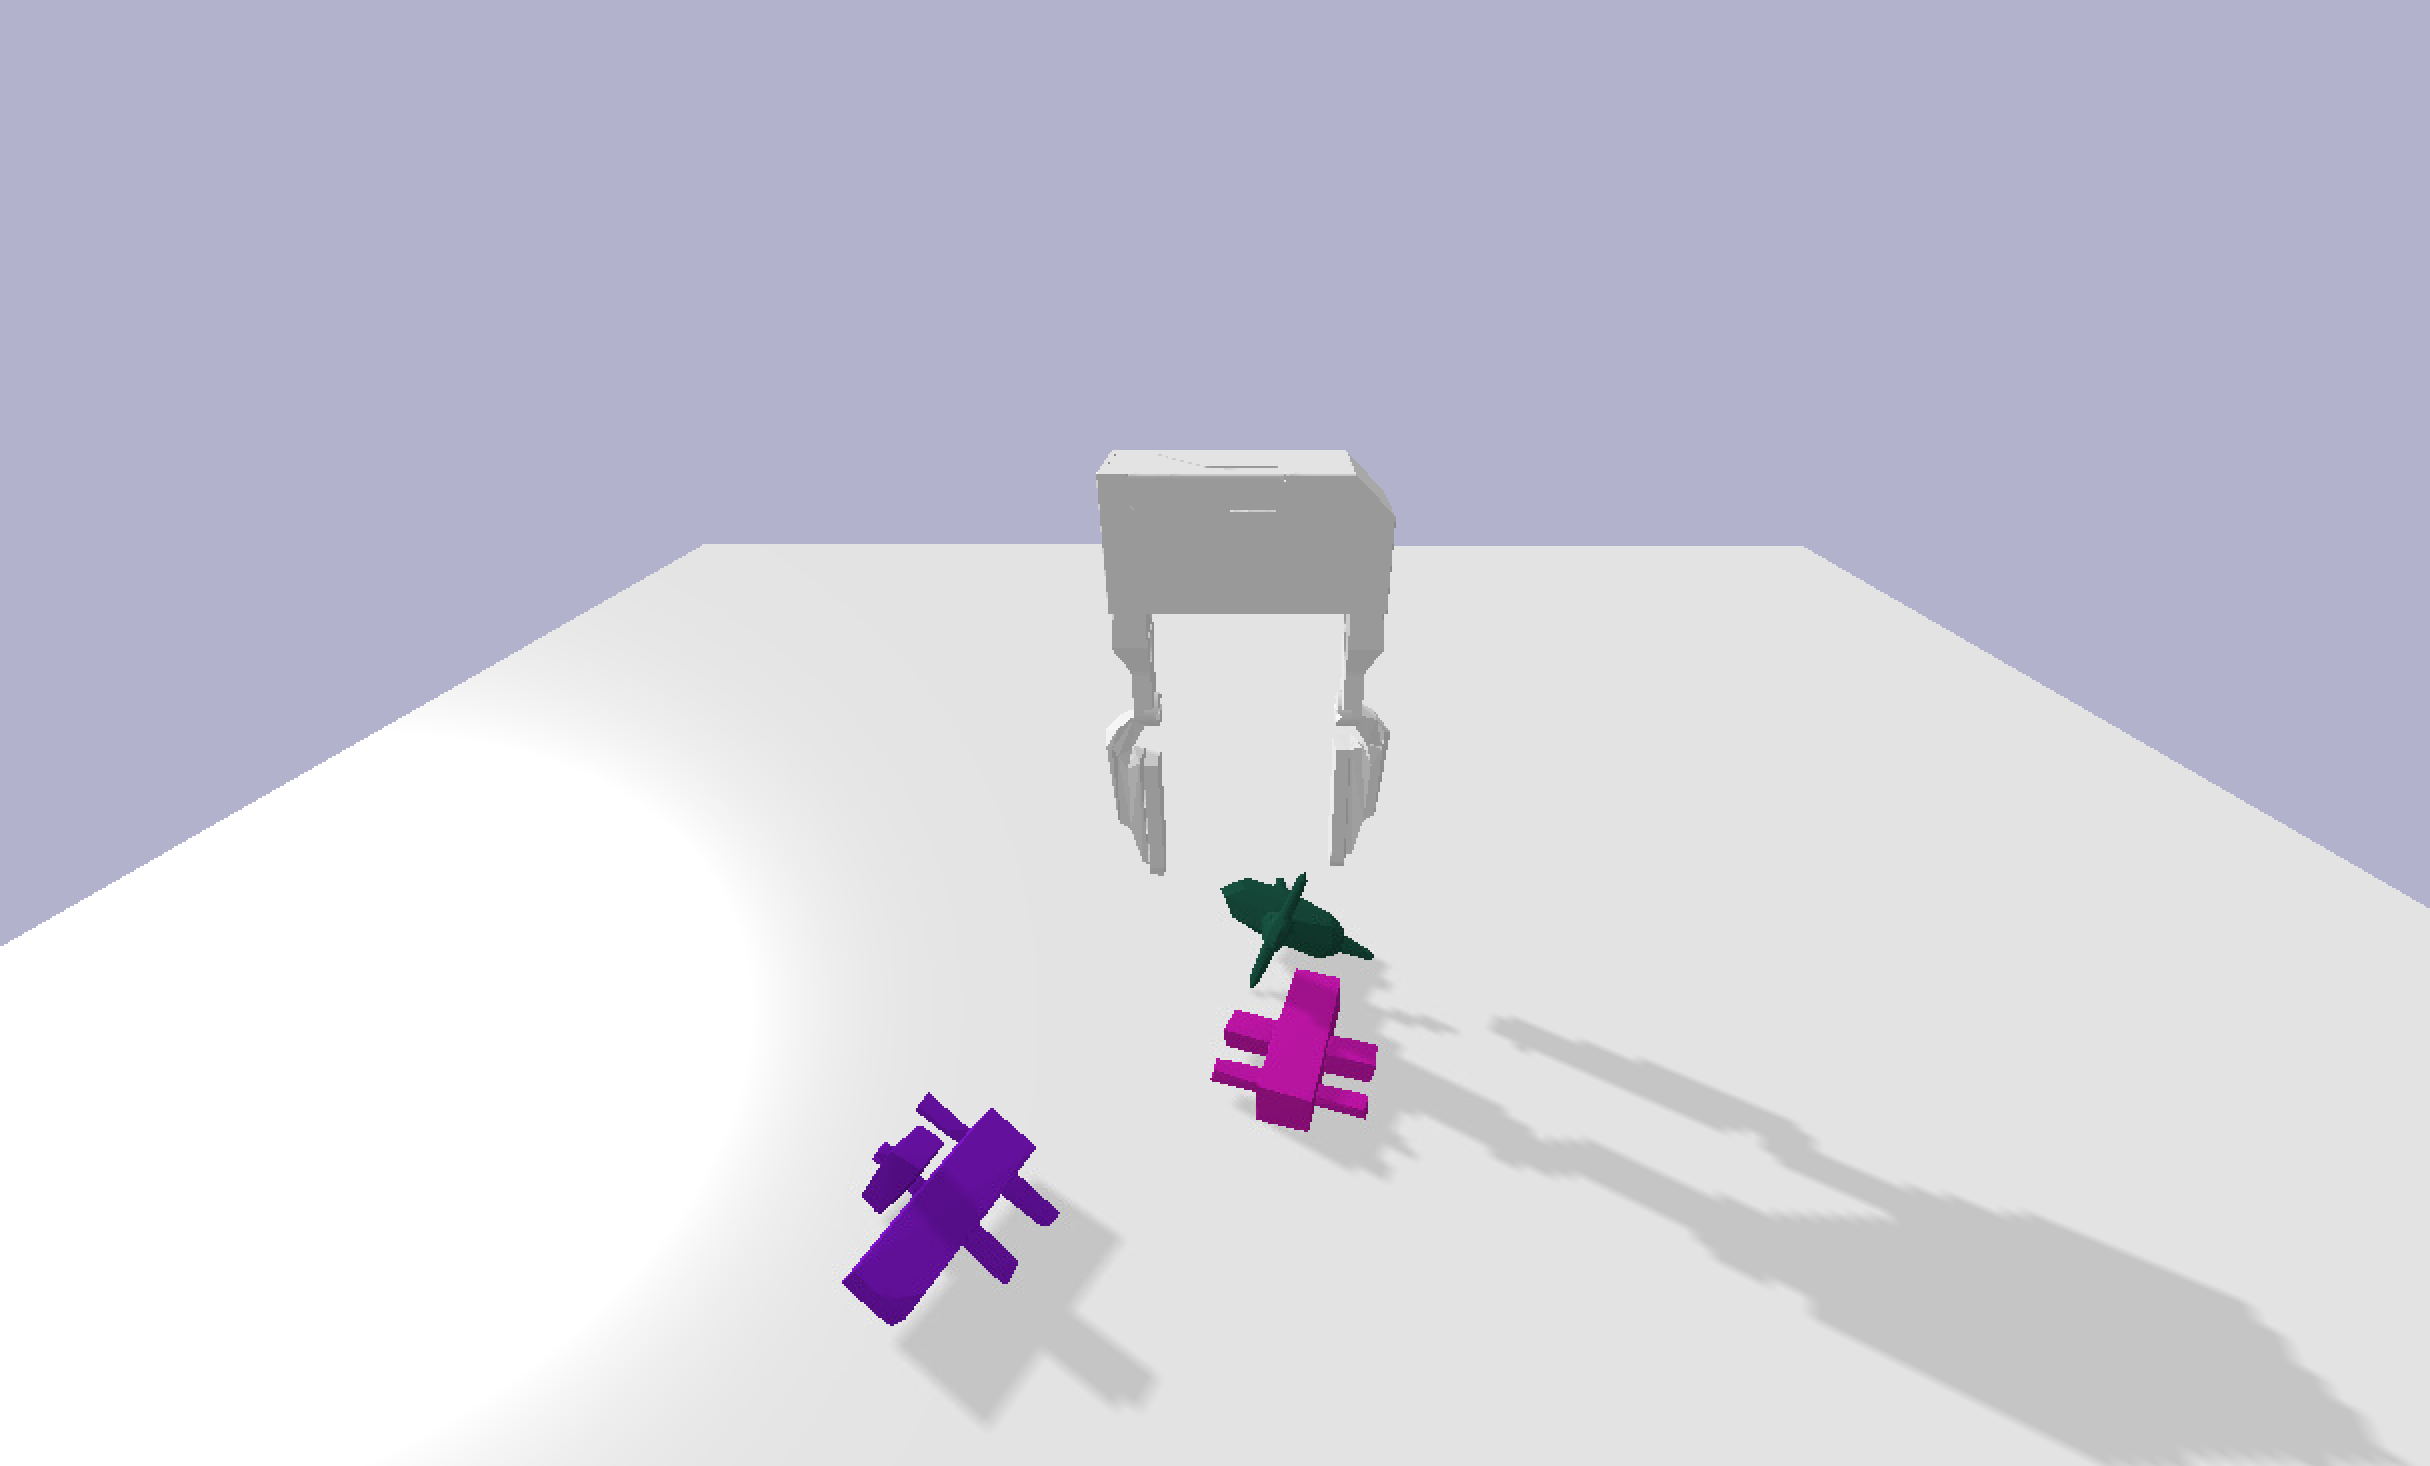
\includegraphics[width=\linewidth]{figures/floor.png}
      \caption{Floor Scene} \label{fig:floor}
    \end{subfigure}%
    \hspace*{\fill}   % maximize separation between the subfigures


\caption{ Table and floor scenes \label{fig:scenes}}
\end{figure}